\documentclass{article}

  % packages
    % basic stuff for rendering math
    \usepackage[letterpaper, top=1in, bottom=1in, left=1in, right=1in]{geometry}
    \usepackage[utf8]{inputenc}
    \usepackage[english]{babel}
    \usepackage{amsmath} 
    \usepackage{amssymb}
    % \usepackage{amsthm}
    \usepackage{bbm}

    % extra math symbols and utilities
    \usepackage{mathtools}        % for extra stuff like \coloneqq
    \usepackage{mathrsfs}         % for extra stuff like \mathsrc{}
    \usepackage{centernot}        % for the centernot arrow 
    \usepackage{bm}               % for better boldsymbol/mathbf 
    \usepackage{enumitem}         % better control over enumerate, itemize
    \usepackage{hyperref}         % for hypertext linking
    \usepackage{fancyvrb}          % for better verbatim environments
    \usepackage{newverbs}         % for texttt{}
    \usepackage{xcolor}           % for colored text 
    \usepackage{listings}         % to include code
    \usepackage{lstautogobble}    % helper package for code
    \usepackage{parcolumns}       % for side by side columns for two column code
    

    % page layout
    \usepackage{fancyhdr}         % for headers and footers 
    \usepackage{lastpage}         % to include last page number in footer 
    \usepackage{parskip}          % for no indentation and space between paragraphs    
    \usepackage[T1]{fontenc}      % to include \textbackslash
    \usepackage{footnote}
    \usepackage{etoolbox}

    % for custom environments
    \usepackage{tcolorbox}        % for better colored boxes in custom environments
    \tcbuselibrary{breakable}     % to allow tcolorboxes to break across pages

    % figures
    \usepackage{pgfplots}
    \pgfplotsset{compat=1.18}
    \usepackage{float}            % for [H] figure placement
    \usepackage{tikz}
    \usepackage{tikz-cd}
  %  \usepackage{circuit-tikz}
    \usetikzlibrary{arrows}
    \usetikzlibrary{positioning}
    \usetikzlibrary{calc}
    \usepackage{graphicx}
    \usepackage{caption} 
    \usepackage{subcaption}

    % for tabular stuff 
    \usepackage{dcolumn}

    \usepackage[nottoc]{tocbibind}
    \pdfsuppresswarningpagegroup=1
    \hfuzz=5.002pt                % ignore overfull hbox badness warnings below this limit

  % New and replaced operators
    \DeclareMathOperator{\Tr}{Tr}
    \DeclareMathOperator{\Sym}{Sym}
    \DeclareMathOperator{\Span}{span}
    \DeclareMathOperator{\std}{std}
    \DeclareMathOperator{\Cov}{Cov}
    \DeclareMathOperator{\Var}{Var}
    \DeclareMathOperator{\Corr}{Corr}
    \DeclareMathOperator{\pos}{pos}
    \DeclareMathOperator*{\argmin}{\arg\!\min}
    \DeclareMathOperator*{\argmax}{\arg\!\max}
    \newcommand{\ket}[1]{\ensuremath{\left|#1\right\rangle}}
    \newcommand{\bra}[1]{\ensuremath{\left\langle#1\right|}}
    \newcommand{\braket}[2]{\langle #1 | #2 \rangle}
    \newcommand{\qed}{\hfill$\blacksquare$}     % I like QED squares to be black

  % Custom Environments
    \newtcolorbox[auto counter, number within=section]{question}[1][]
    {
      colframe = orange!25,
      colback  = orange!10,
      coltitle = orange!20!black,  
      breakable, 
      title = \textbf{Question \thetcbcounter ~(#1)}
    }

    \newtcolorbox[auto counter, number within=section]{exercise}[1][]
    {
      colframe = teal!25,
      colback  = teal!10,
      coltitle = teal!20!black,  
      breakable, 
      title = \textbf{Exercise \thetcbcounter ~(#1)}
    }
    \newtcolorbox[auto counter, number within=section]{solution}[1][]
    {
      colframe = violet!25,
      colback  = violet!10,
      coltitle = violet!20!black,  
      breakable, 
      title = \textbf{Solution \thetcbcounter}
    }
    \newtcolorbox[auto counter, number within=section]{lemma}[1][]
    {
      colframe = red!25,
      colback  = red!10,
      coltitle = red!20!black,  
      breakable, 
      title = \textbf{Lemma \thetcbcounter ~(#1)}
    }
    \newtcolorbox[auto counter, number within=section]{theorem}[1][]
    {
      colframe = red!25,
      colback  = red!10,
      coltitle = red!20!black,  
      breakable, 
      title = \textbf{Theorem \thetcbcounter ~(#1)}
    } 
    \newtcolorbox[auto counter, number within=section]{corollary}[1][]
    {
      colframe = red!25,
      colback  = red!10,
      coltitle = red!20!black,  
      breakable, 
      title = \textbf{Corollary \thetcbcounter ~(#1)}
    } 
    \newtcolorbox[auto counter, number within=section]{proof}[1][]
    {
      colframe = orange!25,
      colback  = orange!10,
      coltitle = orange!20!black,  
      breakable, 
      title = \textbf{Proof. }
    } 
    \newtcolorbox[auto counter, number within=section]{definition}[1][]
    {
      colframe = yellow!25,
      colback  = yellow!10,
      coltitle = yellow!20!black,  
      breakable, 
      title = \textbf{Definition \thetcbcounter ~(#1)}
    } 
    \newtcolorbox[auto counter, number within=section]{example}[1][]
    {
      colframe = blue!25,
      colback  = blue!10,
      coltitle = blue!20!black,  
      breakable, 
      title = \textbf{Example \thetcbcounter ~(#1)}
    } 
    \newtcolorbox[auto counter, number within=section]{code}[1][]
    {
      colframe = green!25,
      colback  = green!10,
      coltitle = green!20!black,  
      breakable, 
      title = \textbf{Code \thetcbcounter ~(#1)}
    } 

    \BeforeBeginEnvironment{example}{\savenotes}
    \AfterEndEnvironment{example}{\spewnotes}
    \BeforeBeginEnvironment{lemma}{\savenotes}
    \AfterEndEnvironment{lemma}{\spewnotes}
    \BeforeBeginEnvironment{theorem}{\savenotes}
    \AfterEndEnvironment{theorem}{\spewnotes}
    \BeforeBeginEnvironment{corollary}{\savenotes}
    \AfterEndEnvironment{corollary}{\spewnotes}
    \BeforeBeginEnvironment{definition}{\savenotes}
    \AfterEndEnvironment{definition}{\spewnotes}
    \BeforeBeginEnvironment{exercise}{\savenotes}
    \AfterEndEnvironment{exercise}{\spewnotes}
    \BeforeBeginEnvironment{proof}{\savenotes}
    \AfterEndEnvironment{proof}{\spewnotes}
    \BeforeBeginEnvironment{solution}{\savenotes}
    \AfterEndEnvironment{solution}{\spewnotes}
    \BeforeBeginEnvironment{question}{\savenotes}
    \AfterEndEnvironment{question}{\spewnotes}
    \BeforeBeginEnvironment{code}{\savenotes}
    \AfterEndEnvironment{code}{\spewnotes}

    \definecolor{dkgreen}{rgb}{0,0.6,0}
    \definecolor{gray}{rgb}{0.5,0.5,0.5}
    \definecolor{mauve}{rgb}{0.58,0,0.82}
    \definecolor{lightgray}{gray}{0.93}

    % default options for listings (for code)
    \lstset{
      autogobble,
      frame=ltbr,
      language=C,                           % the language of the code
      aboveskip=3mm,
      belowskip=3mm,
      showstringspaces=false,
      columns=fullflexible,
      keepspaces=true,
      basicstyle={\small\ttfamily},
      numbers=left,
      firstnumber=1,                        % start line number at 1
      numberstyle=\tiny\color{gray},
      keywordstyle=\color{blue},
      commentstyle=\color{dkgreen},
      stringstyle=\color{mauve},
      backgroundcolor=\color{lightgray}, 
      breaklines=true,                      % break lines
      breakatwhitespace=true,
      tabsize=3, 
      xleftmargin=2em, 
      framexleftmargin=1.5em, 
      stepnumber=1
    }

  % Page style
    \pagestyle{fancy}
    \fancyhead[L]{Measure Theory}
    \fancyhead[C]{Muchang Bahng}
    \fancyhead[R]{Fall 2022} 
    \fancyfoot[C]{\thepage / \pageref{LastPage}}
    \renewcommand{\footrulewidth}{0.4pt}          % the footer line should be 0.4pt wide
    \renewcommand{\thispagestyle}[1]{}  % needed to include headers in title page

\begin{document}

\title{Measure Theory}
\author{Muchang Bahng}
\date{Spring 2024}

\maketitle
\tableofcontents
\pagebreak

This covers computability theory, complexity theory, and automata theory. 
Alphabet. Boolean logic


\section{Sigma Algebras} 

  In here, we will develop a deeper formalism of set theory and topology, now that we have the tools of analysis. 

\subsection{Set-Theroetic Limits}

  Let's talk about sequences of sets $(A_n)_n$. 

  \begin{definition}[Monotone Sequence]
    A sequence of sets $(A_n)_n$ is called 
    \begin{enumerate}
      \item \textbf{(strictly) increasing} if $A_n \subsetneq A_{n+1}$. 
      \item \textbf{nondecreasing} if $A_n \subseteq A_{n+1}$. 
      \item \textbf{(strictly) decreasing} if $A_n \supsetneq A_{n+1}$. 
      \item \textbf{nonincreasing} if $A_n \supseteq A_{n+1}$. 
    \end{enumerate}
  \end{definition}

  \begin{definition}[Limsup and Liminf of Sets]
    Given a sequence of sets $(A_n)_n$, the \textbf{limsup} and \textbf{liminf} of them can be defined in the equivalent ways. 
    \begin{enumerate}
      \item The \textbf{liminf} is the set of points that are missing in only a finite number of sets, and the \textbf{limsup} is the set of points that are in an infinite number of sets. 
      \begin{align}
        \liminf_{n \to \infty} A_n & \coloneqq \bigcup_{n=1}^\infty \bigcap_{m=n}^\infty A_m \\
        \limsup_{n \to \infty} A_n & \coloneqq \bigcap_{n=1}^\infty \bigcup_{m=n}^\infty A_m 
      \end{align} 

      \item The \textbf{liminf} and \textbf{limsup} are the set of points $x$ where the liminf and limsup of the indicator function function evaluated at $x$ equals $1$. 
        \begin{align}
          \liminf_{n \to \infty} A_n & \coloneqq \{x \in X \mid \liminf_{n \to \infty} \mathbbm{1}_{A_n} (x) = 1 \} \\ 
          \limsup_{n \to \infty} A_n & \coloneqq \{x \in X \mid \limsup_{n \to \infty} \mathbbm{1}_{A_n} (x) = 1 \}
        \end{align}

    \end{enumerate}
    Both liminf and limsup always exist for any sequence of sets. 
  \end{definition} 
  \begin{proof}
    DeMorgan's law. 
  \end{proof}

  \begin{lemma}[Monotonicity]
    For any sequence of sets 
    \begin{equation}
      \liminf_{n \to \infty} A_n \subseteq \limsup_{n \to \infty} A_n 
    \end{equation}
  \end{lemma}

  \begin{lemma}[Complements]
    \begin{equation}
      \liminf_{n \to \infty} A_n = \bigg( \limsup_{n \to \infty} A_n^c  \bigg)^c
    \end{equation}
  \end{lemma}
  \begin{proof}
    
  \end{proof}

  \begin{definition}[Limit of Sets]
    
  \end{definition} 

\subsection{Borel Hierarchy}

  \begin{definition}[$F_\sigma$ Sets]
    A \textbf{$F_\sigma$-set} is a subset of a topological space that is a countable union of closed sets. 
  \end{definition}

  \begin{definition}[$G_\delta$ Sets]
    A \textbf{$G_\delta$-set} is a subset of a topological space  that is a countable intersection of open sets. 
  \end{definition}

  \begin{lemma}
    The complement of a $F_\sigma$ set is a $G_\delta$ set. 
  \end{lemma} 

\subsection{Sigma Algebra}

  Now, given any set $X$, we can construct its power set $2^X$. But we can't naively just give a measure to every $A \in 2^X$, since for certain spaces, this causes nasty contradictions shown through the Banach-Tarski Paradox.\footnote{Given any two bounded subsets $A$ and $B$ of $\mathbb{R}^n$ where $n \geq 3$, both of which have a nonempty interior, there are partitions of $A$ and $B$ into a finite number of disjoint subsets, $A = A_1 \cup \ldots \cup A_k$, $B = B_1 \cup \ldots \cup B_k$, such that $A_i$ and $B_i$ are congruent for every $i \in [k]$.} A nice set of subsets of $X$ to work with is the $\sigma$-algebra of $X$. 

  \begin{definition}[$\sigma$-Algebra]
    A \textbf{$\boldsymbol{\sigma}$-algebra} on a set $X$ is a collection  of subsets of $X$, denoted $\mathcal{A} \subset 2^X$ that contains $\emptyset$, $X$ itself, is stable under a countable union, and is stable under complementation. This pair $(X, \mathcal{A})$ is called a \textbf{measurable space}. 
  \end{definition}

  \begin{lemma}[Additional Property of $\sigma$-Algebras]
    A commonly known property of any $\sigma$-algebra $\mathcal{A}$ is that it is stable under countable intersections, too. 
    \begin{equation}
      A_1, A_2, \ldots, \in \mathcal{A} \implies \bigcap_{k=1}^\infty A_k \in \mathcal{A}
    \end{equation}
  \end{lemma}
  \begin{proof}
    We can utilize the fact that 
    \begin{equation}
      \bigcap_{k=1}^\infty A_k = X \setminus \bigcup_{k=1}^\infty A_k^c
    \end{equation}
  \end{proof}

  A $\sigma$-algebra is similar to the topology $\tau$ of topological space. Both $\mathcal{A}$ and $\tau$ require $\emptyset$ and $X$ to be in it. The three differences are that (i) $\tau$ does not allow compelmentation, (ii) $\tau$ allows any (even uncountable) union of sets (condition is strengthened), and (iii) $\tau$ allows only finite intersection of sets (condition is weakened). Now in order to construct $\sigma$-algebras, the following theorems are useful since they allow us to construct $\sigma$-algebras from other $\sigma$-algebras. It turns out that the intersection of $\sigma$-algebras is a $\sigma$-algebra, but not for unions. 

  \begin{theorem}[Intersection of Sigma Algebras is a Sigma Algebra]
    Let $\{\mathcal{A}_k\}$ be a family of $\sigma$-algebras of $X$. Then, $\cap \mathcal{A}_k$ is also a $\sigma$-algebra of $X$. 
  \end{theorem}
  \begin{proof}
    Clearly, $\emptyset, X$ is in $\cap \mathcal{A}_k$. To prove complementation, 
    \begin{equation}
      A \in \bigcap \mathcal{A}_k \implies A \in \mathcal{A}_k \; \forall k \implies A^c \in A_k \; \forall k \implies A^c \in \bigcap \mathcal{A}_k
    \end{equation}
    To prove countable union, let $\{A_j\}_{j \in J}$ be some countable family of subsets in $\cap \mathcal{A}_k$. Then, 
    \begin{equation}
      A_j \in \bigcap \mathcal{A}_k \; \forall j \in J \implies A_j \in \mathcal{A}_k \; \forall k \forall j \implies \bigcup A_j \in \mathcal{A}_k \; \forall k \implies \bigcup A_j \in \bigcap \mathcal{A}_k
    \end{equation}
  \end{proof}

  This allows us to easily prove the following theorem, which just establishes the existence of $\sigma$-algebras. 

  \begin{theorem}[Unique Smallest Sigma Algebra]
    Let $F \subset 2^X$. Then there exists a unique smallest $\sigma$-algebra $\sigma(F)$ containing $F$, called the $\sigma$-algebra \textbf{generated} by $F$. 
  \end{theorem}
  \begin{proof}
    Let us denote $\mathcal{M}$ as the set of all possible $\sigma$-algebras $\mathcal{B}$ of $X$. $\mathcal{M}$ is nonempty since it contains $2^X$. Then, the intersection 
    \begin{equation}
      \bigcap_{\mathcal{B} \in \mathcal{M}} \mathcal{B}
    \end{equation}
    is the unique smallest $\sigma$-algebra. 
  \end{proof} 

  With this guarantee, we can now define what it means for a set of subsets to \textit{generate} a $\sigma$-algebra. 

  \begin{definition}[$\sigma$-Algebra Generated by a Set]
    Given a collection of sets $\mathscr{C}$, the $\sigma$-algebra \textbf{generated} by $\mathscr{C}$ is the unique smallest $\sigma$-algebra containing $\mathscr{C}$, denoted $\sigma(\mathscr{C})$. 
  \end{definition} 

  This gives us a convenient way to construct $\sigma$-algebras. The general method is to identify a collection of ``important'' subsets that we would like to be included in the $\sigma$-algebra, and then just generate it.   

  \begin{definition}[Borel $\sigma$-algebra]
    The \textbf{Borel $\boldsymbol{\sigma}$-algebra} of a topological space $(X, \mathscr{T})$ is the $\sigma$-algebra generated by the topology $\mathscr{T}$, denoted $\mathcal{B}(X) \coloneqq \sigma(\mathscr{T})$. An element of the Borel algebra is called a \textbf{Borel set}. 
  \end{definition}

  Note that the Borel algebra contains: 
  \begin{enumerate}
    \item all open sets, 
    \item all closed sets due to closure under complements, 
    \item all $G_\delta$ sets due to closure under countable unions, 
    \item all $F_\sigma$ sets due to closure under countable intersection. 
  \end{enumerate}

  \begin{definition}[Measure Space]
    A \textbf{measure set} is a tuple $(X, \mathcal{A})$, where $X$ is an arbitrary space and $\mathcal{A}$ a $\sigma$-algebra. 
  \end{definition}

\section{Measures and Sigma Algebras}

  Now, given any set $X$, we can construct its power set $2^X$. But we can't naively just give a measure to every $A \in 2^X$, since for certain spaces, this causes nasty contradictions shown through the Banach-Tarski Paradox. 

  \begin{theorem}[Banach-Tarski Paradox (Strong Form)]
    Given any two bounded subsets $A$ and $B$ of $\mathbb{R}^n$ where $n \geq 3$, both of which have a nonempty interior, there are partitions of $A$ and $B$ into a finite number of disjoint subsets, $A = A_1 \cup \ldots \cup A_k$, $B = B_1 \cup \ldots \cup B_k$, such that $A_i$ and $B_i$ are congruent for every $i \in [k]$. 
  \end{theorem}

  A nice set of subsets of $X$ to work with is the $\sigma$-algebra of $X$. 

  \begin{definition}[$\sigma$-Algebra]
    A \textbf{$\boldsymbol{\sigma}$-algebra} on a set $X$ is a collection  of subsets of $X$, denoted $\mathcal{A} \subset 2^X$ that contains $\emptyset$, $X$ itself, is stable under a countable union, and is stable under complementation. This pair $(X, \mathcal{A})$ is called a \textbf{measurable space}. 
  \end{definition}

  \begin{lemma}[Additional Property of $\sigma$-Algebras]
    A commonly known property of any $\sigma$-algebra $\mathcal{A}$ is that it is stable under countable intersections, too. 
    \begin{equation}
      A_1, A_2, \ldots, \in \mathcal{A} \implies \bigcap_{k=1}^\infty A_k \in \mathcal{A}
    \end{equation}
  \end{lemma}
  \begin{proof}
    We can utilize the fact that 
    \begin{equation}
      \bigcap_{k=1}^\infty A_k = X \setminus \bigcup_{k=1}^\infty A_k^c
    \end{equation}
  \end{proof}

  A $\sigma$-algebra is similar to the topology $\tau$ of topological space. Both $\mathcal{A}$ and $\tau$ require $\emptyset$ and $X$ to be in it. The three differences are that (i) $\tau$ does not allow compelmentation, (ii) $\tau$ allows any (even uncountable) union of sets (condition is strengthened), and (iii) $\tau$ allows only finite intersection of sets (condition is weakened). Now in order to construct $\sigma$-algebras, the following theorems are useful since they allow us to construct $\sigma$-algebras from other $\sigma$-algebras. It turns out that the intersection of $\sigma$-algebras is a $\sigma$-algebra, but not for unions. 

  \begin{theorem}[Intersection of Sigma Algebras is a Sigma Algebra]
    Let $\{\mathcal{A}_k\}$ be a family of $\sigma$-algebras of $X$. Then, $\cap \mathcal{A}_k$ is also a $\sigma$-algebra of $X$. 
  \end{theorem}
  \begin{proof}
    Clearly, $\emptyset, X$ is in $\cap \mathcal{A}_k$. To prove complementation, 
    \begin{equation}
      A \in \bigcap \mathcal{A}_k \implies A \in \mathcal{A}_k \; \forall k \implies A^c \in A_k \; \forall k \implies A^c \in \bigcap \mathcal{A}_k
    \end{equation}
    To prove countable union, let $\{A_j\}_{j \in J}$ be some countable family of subsets in $\cap \mathcal{A}_k$. Then, 
    \begin{equation}
      A_j \in \bigcap \mathcal{A}_k \; \forall j \in J \implies A_j \in \mathcal{A}_k \; \forall k \forall j \implies \bigcup A_j \in \mathcal{A}_k \; \forall k \implies \bigcup A_j \in \bigcap \mathcal{A}_k
    \end{equation}
  \end{proof}

  This allows us to easily prove the following proposition, which just establishes the existence of $\sigma$-algebras. 

  \begin{proposition}[Unique Smallest Sigma Algebra]
    Let $F \subset 2^X$. Then there exists a unique smallest $\sigma$-algebra $\sigma(F)$ containing $F$, called the $\sigma$-algebra \textbf{generated} by $F$. 
  \end{proposition}
  \begin{proof}
    Let us denote $\mathcal{M}$ as the set of all possible $\sigma$-algebras $\mathcal{B}$ of $X$. $\mathcal{M}$ is nonempty since it contains $2^X$. Then, the intersection 
    \begin{equation}
      \bigcap_{\mathcal{B} \in \mathcal{M}} \mathcal{B}
    \end{equation}
    is the unique smallest $\sigma$-algebra. 
  \end{proof}

  Now, we can introduce the first nontrivial $\sigma$-algebra, called the Borel $\sigma$-algebra. 

  \begin{definition}[Borel $\sigma$-algebra]
    The \textbf{Borel $\boldsymbol{\sigma}$-algebra} of a topological space $(X, \mathscr{T})$ is the $\sigma$-algebra generated by the topology $\mathscr{T}$, denoted $\mathcal{B}(X) \coloneqq \sigma(\mathscr{T})$. 
  \end{definition} 

  \begin{definition}[Limsup and Liminf of Sets]
    Given a collection of sets $(A_n)_n$, we can define the limsup and liminf of a sequence of them. 
    \begin{enumerate}
      \item All points that are missing in only a finite number of sets. 
        \begin{equation}
          \liminf A_n \coloneqq \bigcup_{n=1}^\infty \bigcap_{m=n}^\infty A_m 
        \end{equation}

      \item All points that are in an infinite number of sets 
        \begin{equation}
          \limsup A_n = \bigcap_{n=1}^\infty \bigcup_{m=n}^\infty A_m 
        \end{equation}
    \end{enumerate}
  \end{definition}

  Now, how do we measure a size on $\mathcal{B}(X)$? We use measures. 

  \begin{definition}[Measure]
    Given a measurable space $(X, \mathcal{A})$, a \textbf{measure} is a function $\mu : \mathcal{A} \longrightarrow [0, +\infty]$ satisfying 
    \begin{enumerate}
      \item Null empty set $\mu(\emptyset) = 0$ 
      \item Countable additivity: For all countable collections $\{A_k\}_{k=1}^\infty$ of pairwise disjoint subsets $A_k \in \mathcal{A}$, 
      \begin{equation}
        \mu \bigg( \bigsqcup_{k=1}^\infty A_k \bigg) = \sum_{k=1}^\infty \mu(A_k)
      \end{equation}
      Remember that we are allowed to take countable unions inside our $\sigma$-algebra, so this makes sense. 
    \end{enumerate}
    This immediately implies that given $A, B \in \mathcal{A}$, then $A \subset B \implies \mu(A) \leq \mu(B)$. The triplet $(X, \mathcal{A}, \mu)$ is called a \textbf{measure space}. 
  \end{definition}

  The first condition is important because it allows us to take finite disjoint unions. That is, since $\mu(A_1 \cup A_2) = \mu(A_1 \cup A_2 \cup \emptyset \cup \ldots)$, we have 
  \begin{equation}
    \sum_{k=1}^\infty = \mu(A_1) + \mu(A_2)
  \end{equation}
  Disjointness is clearly important since if it wasn't, then $\mu(A) = \mu(A \cup A) = 2 \mu(A)$, which is absurd. Now our natural measure on the real number line with its Borel $\sigma$-algebra $(\mathbb{R}, \mathcal{B})$, we want a measure satisfying $\mu((a, b)) = b - a$ and $\mu([0, \infty)) = \infty$. Such a measure does exist, and it is called the Lebesgue measure, but proving its existence is highly nontrivial. Let us first look into some properties of measures, which all seem natural. 

  \begin{proposition}
    If $A_1 \subset A_2 \subset A_3 \subset \ldots$, then 
    \begin{equation}
      \mu\bigg( \bigcup_{k=1}^\infty A_k \bigg) = \lim_{k \rightarrow \infty} \mu(A_k)
    \end{equation}
  \end{proposition}
  \begin{proof}
    This is the first time we introduce limits. With the fact that $\mu(A_k)$ must be nondecreasing, we can use real analysis and see that it is bounded by $\infty$, meaning that it must have a limit. But why does this limit equal to the left hand side? We can see that 
    \begin{align}
      \mu\bigg( \bigcup_{k=1}^\infty A_k \bigg) & = \mu(A_1) + \sum_{k=2}^\infty \mu(B_k) \\
      & = \mu(A_1) + \lim_{k \rightarrow \infty} \sum_{k=2}^\infty \mu(B_k) \\
      & = \lim_{k \rightarrow \infty} \mu(A_1 \cup B_2 \cup \ldots B_k)  = \lim_{k \rightarrow \infty} \mu(A_k) 
    \end{align}
    where $B_k = A_k \setminus A_{k-1}$. 
  \end{proof}

  Now a similar theorem, but with a little twist to it. 

  \begin{proposition}
    If $A_1 \supset A_2 \supset A_3 \supset \ldots$, then 
    \begin{equation}
      \mu\bigg( \bigcap_{k=1}^\infty A_k \bigg) = \lim_{k \rightarrow \infty} \mu(A_k)
    \end{equation}
    if $\mu(A_1) < \infty$. 
  \end{proposition}
  \begin{proof}
    The $\mu(A_1) < \infty$ is a necessary condition, since if we take $A_k = [k, \infty)$ on the real number line, then we have $\cap_{k=1}^\infty A_k = \emptyset$, but the limit of the measure is $\infty$. Well we can define $B_k = A_k \setminus A_{k+1}$ and write $\cap_{k=1}^\infty A_k = A_1 \setminus \cup_{k=1}^\infty B_k$, which means that 
    \begin{align*}
      \mu\bigg( \bigcap_{k=1}^\infty A_k \bigg) & = \mu\bigg( A_1 \setminus \bigcup_{k=1}^\infty B_k \bigg) \\
      & = \mu(A_1) - \mu\bigg( \bigcup_{k=1}^\infty B_k\bigg) \\
      & = \mu(A_1) - \sum_{k=1}^\infty \mu(B_k) \\
      & = \mu(A_1) - \lim_{K \rightarrow \infty} \sum_{k=1}^K \mu(B_k) \\
      & = \lim_{K \rightarrow \infty} \bigg( \mu(A_1) - \sum_{k=1}^K \mu(B_k) \bigg) \\
      & = \lim_{K \rightarrow \infty} \mu \bigg( A_1 \setminus \bigcup_{k=1}^K B_k \bigg) = \lim_{K \rightarrow \infty} \mu(A_K)
    \end{align*}
    Now the first line uses the fact that if $A \subset B$, then $\mu(B \setminus A) + \mu(A) = \mu(B)$, and with the further assumption that $\mu(A) < \infty$, we can subtract on both sides like we do with regular arithmetic. 
  \end{proof}

\subsection{Outer Measures, Construction of Lebesgue Measure}

  Now let's try to construct a measure $\lambda$ on the Borel $\sigma$-algebra $\mathcal{B}(\mathbb{R})$ that assigns length, i.e. $\lambda([a, b]) = b - a$. We will do so by constructing outer measures $\lambda^*: 2^\mathbb{R} \longrightarrow \mathbb{R}$ that acts on the power set of $\mathbb{R}$ s.t. $\lambda^*([a, b]) = b - a$. But this turns out to have its own problems and contradictions, so once we construct such a $\lambda^*$, we will "throw away" all the sets that don't behave nicely under $\lambda^*$ and just use its restriction on the Borel algebra. It turns out that the sets that do behave well under $\lambda^*$ is bigger than the Borel algebra, call it $\mathcal{M}_{\lambda^*}$. So, we have $\mathcal{B}(\mathbb{R}) \subset \mathcal{M}_{\lambda^*} \subset 2^\mathbb{R}$. We will do this in full generality in the following way. We take any space $X$ and construct an outer measure $\mu^*$ on its power set $2^X$. Then, we construct the $\sigma$-algebra of well-behaved sets $\mathcal{M}_{\mu^*} \subset 2^X$, and define our measure $\mu$ on $\mathcal{M}_{\mu^*}$. When defining our outer measure, the condition that the outer measure of a disjoint union of subsets is equal to the sum of the outer measure of the subsets is a bit too restricting, so we use a softer condition. 

  \begin{definition}[Outer Measure]
    A function $\mu^* : 2^X \longrightarrow [0, \infty]$ is an \textbf{outer measure} if $\mu^*(\emptyset) = 0$, $A \subset B \implies \mu^* (A) \leq \mu^*(B)$, and 
    \begin{equation}
      \mu^* \bigg( \bigcup_{k=1}^\infty A_k \bigg) \leq \sum_{k=1}^\infty \mu^* (A_k)
    \end{equation}
    This final condition removes the fact that they must be disjoint, and now we have an inequality. 
  \end{definition}

  Now to construct our Lebesgue outer measure, let us define the following on $\mathbb{R}$. It's a hard definition, but a natural one, since we're taking all these intervals and trying to make them as snug as possible to define the outer measure of an arbitrary set. 

  \begin{definition}[Lebesgue Outer Measure of $\mathbb{R}$]
    Given $A \subset \mathbb{R}$, let 
    \begin{equation}
      C_A = \big\{ \{(a_j, b_j)\}_{j=1}^\infty \mid A \subset \bigcup_{j=1}^\infty (a_j, b_j) \big\}
    \end{equation}
    This is more complicated than it looks. Given a set $A$, we are looking at a family of all collections of intervals that cover $A$. Clearly, all coverings in $C_A$ must have a length greater than $A$, and their length can be easily measured by summing up the intervals $\sum_{j=1}^\infty (b_j - a_j)$. So, we can define the outer measure of $A$ to be the infimum of these sums. 
    \begin{equation}
      \lambda^*(A) = \inf_{C_A} \sum_{j=1}^\infty (b_j - a_j)
    \end{equation}
    We can also generalize this further by introducing a increasing, continuous function $F: \mathbb{R} \rightarrow \mathbb{R}$ and defining the outer measure to be 
    \begin{equation}
     \lambda^*(A) = \inf_{C_A} \sum_{j=1}^\infty \big( F(b_j) - F(a_j) \big) 
    \end{equation}
  \end{definition}

  \begin{example}[Rationals have Outer Measure $0$]
    Let us prove that $\lambda^*(\mathbb{Q}) = 0$. It is countable so we can enumerate it $\mathbb{Q} = \{ q_j\}_{j=1}^\infty$. This is counterintuitive, because since $\mathbb{Q}$ is dense in $\mathbb{R}$, in order to make a covering of $\mathbb{Q}$ we sort of have to cover the entire real line. Visually, this is hard, but it is pretty simple to show that you don't have to. We pick $\epsilon > 0$ and define 
    \begin{equation}
      I_j = \big( q_j - \frac{\epsilon}{2^j} , q_j + \frac{\epsilon}{2^j} \big)
    \end{equation}
    So, 
    \begin{equation}
      \sum_{j=1}^\infty |I_j| = \sum_{j=1}^\infty \frac{\epsilon}{2^j} = 2 \epsilon
    \end{equation}
    This collection $\{I_j\}$ is one element of $C_\mathbb{Q}$ of coverings of the rationals, and taking $\epsilon$ as small as we want, the infimum is $0$. This can be done with all countable subsets of $\mathbb{R}$. 
  \end{example}

  \begin{definition}[Almost Everywhere]
    Given a measure space $(X, \mathcal{A}, \mu)$, a subset $A \in \mathcal{A}$ is said to be a $\mu$-null set if $\mu(A) = 0$. If some property holds for all points $x \in X$ except on a null set, then we say that the property holds \textbf{almost everywhere}.
  \end{definition}

  \begin{example}[Rational Function]
    The function $f(x) = \frac{1}{\sqrt{|x|}}$ is less than $\infty$ almost everywhere. 
  \end{example}

  \begin{proposition}[$\lambda^*$ is an Outer Measure]
    The first condition is trivial. As for 2, if I have $A \subset B \subset \mathbb{R}$ and have a covering of $B$, then I also have a covering of $A$, and so the infimum corresponding to the covering of $B$ must be greater than or equal to the infimum of that corresponding to the covering of $A$. For 3, we want to prove that the outer measure of the union of $A_k$'s is less than or equal to the sum of the outer measures of the $A_k$'s. We pick $\epsilon > 0$ and have some covering $\{(a^k_j, b^k_j)\}_{j=1}^\infty \in C_{A^k}$. So we have 
    \begin{equation}
      \lambda^*(A_k) \leq \sum_{j=1}^\infty b^k_j - a^k_j
    \end{equation}
    We want the inequality to go the other way around, but we can't do that. But note that $\lambda^* (A_k)$ is the infimum of all coverings $\{(a^k_j, b^k_j)\}_{j=1}^\infty$ of $A_k$, and so we can choose a covering that is as close to $\lambda^* (A_k)$, and then add a term of $\epsilon$ to $\lambda^*(A_k)$ to make it greater than this covering. This is an important step of the proof that is used often! 
    \begin{equation}
      \frac{\epsilon}{2^k} + \lambda^* (A_k) \geq \sum_{j=1}^\infty b_j^k - a_j^k 
    \end{equation}
    Now, 
    \begin{equation}
      A = \bigcup_{k=1}^\infty A_k \subset \bigcup_{k=1}^\infty \bigcup_{j=1}^\infty (a_j^k, b_j^k)
    \end{equation}
    and we can see that $\{(a_j^k , b_j^k)\}_{j, k=1}^\infty \in C_A$ is a countable covering of $A$ (since the countable union of a countable union is countable), implying that 
    \begin{equation}
      \lambda^* (A) \leq \sum_{k=1}^\infty \sum_{j=1}^\infty (b_j^k - a_j^k) \leq \sum_{k=1}^\infty \bigg( \lambda^* (A_k) + \frac{\epsilon}{2^k} \bigg) = \epsilon + \sum_{k=1}^\infty \lambda^*(A_k)
    \end{equation}
    and so setting $\epsilon$ arbitrarily small we have $\lambda^* (A) \leq \sum_{k=1}^\infty \lambda^* (A_k)$. 
  \end{proposition}

  In $\mathbb{R}^n$, this construction is exactly the same, since we can take rectangular prisms, which we know the area/volume of, make a countable covering of some arbitrary set $A \subset \mathbb{R}^n$, and then find the infimum of the volume of this set. But we can't apply the outer measure on power sets since there exists some sets that do not behave like how we want it to behave under a measure. For example, there exists disjoint $A, B \subset (0, 1)$ s.t. $A \cup B = (0, 1)$, but $\lambda^*(A) + \lambda^*(B) > 1$. 

  \begin{definition}[Carathéodory's criterion]
    Given outer measure $\mu^*$ on $X$, a set $B$ is $\mu^*$-measurable if 
    \begin{equation}
      \forall A \subset X \; \mu^*(A) = \mu^*(A \cap B) + \mu^*(A \cap B^c)
    \end{equation}
    Obviously, the LHS $\leq$ RHS by the third condition of outer measures. 
  \end{definition}

  There is not much of an intuition for this definition, but in general it says that no matter how nasty a subset $A$ is, $B$ should be nice enough that we can cut $B$ into two pieces. Remember that this is a condition on $B$, not $A$. 

  \begin{example}
    Take $X = \mathbb{R}$ and have $B = (-\infty, b]$. Then $B^c = (b, \infty)$, and $B$ divides $\mathbb{R}$ into a right side and a left side. If we take any subset $A \subset \mathbb{R}$, then $B$ is nice enough to divide $A$ into a left and a right side. 
  \end{example}

  \begin{theorem}
    If $\mu^*$ is an outer measure on $X$, $\mathcal{M}_{\mu^*} = \{$all $\mu^*$-measurable sets$\}$, then 
    \begin{enumerate}
      \item $\mathcal{M}_{\mu^*}$ is a $\sigma$-algebra. 
      \item $\mu = \mu^* \big|_{\mathcal{M}_{\mu^*}}$ is a measure. 
    \end{enumerate}
  \end{theorem}

  To recap, we first take a set $X$, construct an outer measure $\mu^*$ on it. This allows us to define the set of all $\mu^*$-measurable sets $B$ on $X$, which create a $\sigma$-algebra $\mathcal{M}$, and the restriction of $\mu^*$ onto $\mathcal{M}$ is a measure $\mu$. For $\mathbb{R}$, we can create our Lebesgue outer measure $\lambda^*$ on it, which generates the Lebesgue $\sigma$-algebra $\mathcal{M}_{\lambda^*}$. This turns out to be bigger than the Borel $\sigma$-algebra $\mathcal{B}(\mathbb{R})$, but there is little difference in which one we choose when we actually integrate. 

  \begin{theorem}
    A set $E \subset \mathbb{R}$ is Lebesgue measurable implies that it is also Borel measurable. 
    \begin{equation}
      \mathcal{B}(\mathbb{R}) \subset \mathcal{M}_{\lambda^*} \subset 2^\mathbb{R}
    \end{equation}
  \end{theorem}

  \begin{lemma}
    If $E \subset \mathbb{R}$ and $\lambda^*(E) = 0$, then $E \in \mathcal{M}_{\lambda^*}$, i.e. $E$ is Lebesgue outer-measurable. 
  \end{lemma}
  \begin{proof}
    We must prove that $E$ satisfies the Carathéodory's criterion. For all $E \subset \mathbb{R}$, we know that $\lambda^*(A) \leq \lambda^*(A \cap E) + \lambda^*(A \cap E^c)$ by definition of outer measure. Now, since $\lambda^* (E) =0$ and $A \cap E \subset E$, this means that $\lambda^* (A \cap E) = 0$ also. Furthermore, $A \cap E^c \subset A$, meaning that $\lambda^*(A) \geq \lambda^* (A \cap E^c)$, and we get 
    \begin{equation}
      \lambda^*(A) \geq \lambda^*(A \cap E) + \lambda^*(A \cap E^c)
    \end{equation}
    which proves equality. 
  \end{proof}

  Now there are nice properties that we want Lebesgue measures to have: completeness, regularity, and translation invariance. 
  \begin{enumerate}
    \item Completeness: Given sets $A \subset B \subset C$ with $\mu(A) = \mu(C)$ and $A, C \in \mathcal{A}$, this implies that $B \in \mathcal{A}$. This basically says that if you a set that is squeezed in between two measurable sets of equal measure, then the middle set will also be measurable. 
    \item Regularity: Given sets $A \subset B \subset C$, regularity talks about whether I can approximate $B$ well. Must nice measures have this property. 
      \begin{equation}
      \sup_{A \text{ compact}} \mu(A) = \mu(B) = \inf_{C \text{ open}} \mu(C)
      \end{equation}
    \item Translation invariance: Lebesgue measure is translation invariant. $\mu(x + A) = \mu(A)$ for all $x \in \mathbb{R}^n$ on $\mathcal{B}(\mathbb{R}^n)$. 
  \end{enumerate}


\section{Measurable Functions}

  So far, we have defined measurable sets, constructed the Lebesgue measure, and shown that Lebesgue measurable sets can be approximated by nice open sets. Now, let's talk about measurable functions. Just like for measurable sets, there is a general sense in which we can define them and there is the more ``Euclidean'' way of defining them. 

  \begin{definition}[Measurable Function]
    Given a measurable space $(X, \mathcal{A})$, $f: (X, \mathcal{A}) \longrightarrow \mathbb{R}$ is \textbf{measurable} if 
    \begin{equation}
      f^{-1}(A) \in \mathcal{A} \text{ for all } A \text{ open}
    \end{equation}
    Note that measurable functions are always defined on measurable sets, so we don't have to state that its domain is always measurable. 
  \end{definition}

  \begin{theorem}[Measurable Functions on Real Line]
    Let $f: E \subset \mathbb{R} \to \mathbb{R} \cup \{ \pm \infty\}$ and $E$ be measurable. Then, TFAE 
    \begin{enumerate} 
      \item $\forall c \in \mathbb{R}$, $\{x \in E \mid f(x) > c\}$ is measurable. 
      \item $\forall c \in \mathbb{R}$, $\{x \in E \mid f(x) \geq c\}$ is measurable. 
      \item $\forall c \in \mathbb{R}$, $\{x \in E \mid f(x) < c\}$ is measurable. 
      \item $\forall c \in \mathbb{R}$, $\{x \in E \mid f(x) \leq c\}$ is measurable. 
      \item $f$ is Lebesgue measurable. 
    \end{enumerate}
    Furthermore, if any of these hold, then also $\{x \in E \mid f(x) = c \}$ is measurable for all $c$ (but not the converse!). 
  \end{theorem} 
  \begin{proof}
    We know that $(1) \iff (4)$ and $(2) \iff (3)$ by taking complements. We prove $(1) \iff (2)$. 
    \begin{enumerate}
      \item $(1) \implies (2)$. 
      \begin{equation}
        \{x \in E \mid f(x) \geq c \} = \bigcap_{k=1}^\infty \{x \in E \mid f(x) > c - \frac{1}{k} \}
      \end{equation}

      \item $(2) \implies (1)$. 
      \begin{equation}
        \{ x \in E \mid f(x) > c\} = \bigcup_{k=1}^\infty \{x \in E \mid f(x) \geq c + \frac{1}{k} \}
      \end{equation}
    \end{enumerate}

    For $(5)$, we know that
    \begin{enumerate}
      \item $(5) \implies (1)$ is trivial, since open intervals are open sets. 
      \item $(1) \implies (5)$. Any open set is a countable union of disjoint open intervals, and so let 
      \begin{equation}
        U = \bigcup_{k=1}^\infty I_k, \qquad I_k = (a_k, b_k) = \underbrace{(-\infty, b_k)}_{B_k} \cap \underbrace{(a_k, +\infty)}_{A_k}
      \end{equation} 
      Therefore, 
      \begin{equation}
        f^{-1} (U) = \bigcup_{k=1}^\infty f^{-1} (B_k \cap A_k) = \bigcup_{k=1}^\infty \{f^{-1} (B_k) \cap f^{-1} (A_k) \}
      \end{equation}
      which is measurable since countable union/intersections are measurable (by definition of $\sigma$-algebra). 
    \end{enumerate}

    For the final implication, we can use $(2)$ and $(4)$ to get 
    \begin{equation}
      \{x \in E \mid f(x) = c\} = \{x \in E \mid f(x) \leq c \} \cup \{x \in E \mid f(x) \geq c \}
    \end{equation}
  \end{proof} 

  The first question is how you would relate this to continuity. 

  \begin{theorem}[Continuous Functions are Measurable]
    If $f: X \to \mathbb{R}$ is continuous, then it is measurable. 
  \end{theorem}
  \begin{proof}
    If $f$ is continuous, then $f^{-1} (O) = U \cap X$ for every open $O$ with open $U$. 
  \end{proof}

  \begin{theorem}[Monotonic Functions are Measurable] 
    Let $I$ be an interval. If $f: I \subset \mathbb{R}$ is monotone, then $f$ is measurable.
  \end{theorem}
  \begin{proof}
    You can probably see that it is more advantageous to prove using the definition of measurability using rays. We wish to show that for all $c$, $E_c \coloneqq \{x \in I \mid f(x) > c\}$ is measurable. We wish to show that $E_c$ is an interval, though there seems to be some complications with potential discontinuities. 

    Therefore, we use an equivalent definition of an interval: $I$ is an interval if for every $x, y \in I$, $x < t < y \implies t \in I$. Therefore, we can see that if $x, y \in E_c$, then $f(x) > c, f(y) > c$. Therefore, if $t$ is in between them, $f(t) > f(\min\{x, y\}) > c$, and so $t \in E_c$. Since intervals are measurable, we are done. 
  \end{proof}

  There is also some notion of robustness. 

  \begin{theorem}[Function Difference on Measure 0 Set Doesn't Affect Measurability]
    Suppose $f: E \subset \mathbb{R} \to \mathbb{R} \cup \{\pm \infty\}$ with $E$ measurable, and let $g$ be some other function. If $f$ is measurable on $E$ and $g(x) = f(x)$ a.e. for $x \in E$, then $g$ is measurable on $E$. 
  \end{theorem}
  \begin{proof}
    We wish to show that for any open $O \subset \mathbb{R}$, $g^{-1} (O)$ is measurable. We might start with Carathéodory and try to show that for all $A \subset E$, 
    \begin{equation}
      m^\ast(A) = m^\ast (A \cap g^{-1}(O)) + m^\ast (A \cap g^{-1}(O)^c)
    \end{equation}
    But this turns out to be overkill. Since this is about $0$ measure sets, you should be thinking about how $0$-measure sets do not affect measurability and try to use this. In $g^{-1}(O)$, there is a portion of it that overlaps with $f$---call it $A \subset E$---and a portion that doesn't. We know that $m^\ast (E \setminus A) = 0$\footnote{TBD: Can we write $m$? } and a measure $0$ set difference doesn't affect measurability, so $A$ is measurable. So let's decompose it. 
    \begin{align}
      g^{-1} (O) & = \big( g^{-1} (O) \cap A \big) \cup \big( g^{-1} (O) \cap (E \setminus A) \big) \\ 
                 & = \big( f^{-1} (O) \cap A \big) \cup \big( g^{-1} (O) \cap (E \setminus A) \big)
    \end{align}
    If we try to take the measure of this, the first term is the union of measurable sets $f^{-1} (O)$ and $A$. The second term is also measurable since the outer measure is $0$, by subadditivity compared to $m^\ast(E \setminus A) = 0$. Therefore $g^{-1} (O)$ is measurable. 
  \end{proof}
  \begin{proof}
    In class. Consider $S = \{x \in E \mid g(x) < c \}$. Let $A \subset E$ be the set where $g(x) = f(x)$, with $m (E \setminus A) = 0$. Then, 
    \begin{equation}
      S = \big( \{x \in E \mid g(x) < c\} \cap (E \setminus A) \big) \cup \big( \{x \in E \mid f(x) < c\} \cap A \big) 
    \end{equation}
    where the first term is measure $0$ by monotonicity with $E \setminus A$, $m(E \setminus A) = 0$, and the second term is measurable since $A = E \setminus (E \setminus A)$. So, $S$ is measurable. 
  \end{proof}

  You preserve measurability if you split the domain in a ``measurable way.'' 

  \begin{theorem}[Measurable Partition Induces Measurable Restrictions of Functions]
    Take a measurable subset $D \subset E$ and let $f: E \to \mathbb{R} \cup \{\pm\infty\}$ be a function. Then, the following are equivalent. 
    \begin{enumerate}
      \item $f$ is measurable on $E$ 
      \item $f$ is measurable on $D$ and on $E \setminus D$. 
    \end{enumerate}
  \end{theorem}
  \begin{proof}
    We prove bidirectionally. 
    \begin{enumerate}
      \item $(\rightarrow)$. Let's prove measurability on $D$. We can see that 
      \begin{equation}
        \{x \in D \mid f(x) \in O \} = \{x \in E \mid f(x) \in O \} \cap D
      \end{equation}
      as the intersection of measurable sets, is measurable. Then we can just take the complement of both sides to get. 
      \begin{align}
        \{x \in E \setminus D \mid f(x) \in O\} 
          & = E \setminus \{x \in D \mid f(x) \in O \} \\ 
          & = E \setminus \big( \{x \in E \mid f(x) \in O \} \cap D \big) \\
          & = \underbrace{\big( E \setminus \{x \in E \mid f(x) \in O \} \big)}_{\text{measurable}} \cup \underbrace{\big( E \setminus D \big)}_{\text{measurable}}
      \end{align}
      which is also measurable. 

      \item $(\leftarrow)$. Take some open $O \subset \mathbb{R} \cup \{\pm\infty\}$ and take its preimage. Then, 
      \begin{equation}
        f^{-1} (O) = \{x \in D \mid f(x) \in O\} \cup \{x \in E \setminus D \mid f(x) \in O \}
      \end{equation} 
      as the finite union and intersection of measurable sets, is measurable. 
    \end{enumerate}
  \end{proof}

\subsection{Arithmetic and Composition of Measurable Functions}

  The following theorem is useful, since we don't want to manually check measurability of every single new function we create. 

  \begin{theorem}[Arithmetic on Measurable Functions]
    Given measurable functions $f, g: E \subset \mathbb{R} \to \mathbb{R}$, the following standard operations on them create new measurable functions: 
    \begin{enumerate}
      \item $\alpha f$ is measurable for all $\alpha \in \mathbb{R}$. 
      \item $f + g$ is measurable 
      \item $f \cdot g$ is measurable 
      \item $f / g$ is measurable on $\{x \mid g(x) \neq 0\}$ 
    \end{enumerate}
  \end{theorem} 
  \begin{proof}
    WLOG, we can assume $f, g$ are finite everywhere since changing these values to finite values over a set of measure $0$ doesn't affect measurability. 
    \begin{enumerate}
      \item If $\alpha = 0$, this is trivially true. If not, then 
      \begin{equation}
        \{ x \in E \mid (\alpha f) (x) < c \} = \{x \in E \mid f(x) < \frac{c}{\alpha} \} 
      \end{equation}

      \item Suppose $f(x) + g(x) < c \iff f(x) < c - g(x) \iff \exists q \in \mathbb{Q}$ s.t. $f(x) < q < c - g(x)$.\footnote{The reason we want to introduce rationals is that we want to take advantage of countability.} Then, 
      \begin{equation}
        \{x \in E \mid f(x) + g(x) < c \} = \bigcup_{q \in \mathbb{Q}} \big( \{x \in E \mid f(x) < q\} \cap \{x \in E \mid g(x) < c - q \}\big)
      \end{equation}
      which is a countable union of measurable sets, and is measurable. 

      \item We use a nice trick from analysis. 
      \begin{equation}
        fg = \frac{1}{4} \big( (f + g)^2 - (f - g)^2 \big) 
      \end{equation}
      and so it suffices to prove that $h$ measurable implies $h^2$ measurable. For $c \geq 0$\footnote{We only need to consider this case since $h^2$ is always nonnegative and so $c < 0$ would mean preimage is empty set.}, we have 
      \begin{equation}
        \{ x \in E \mid h^2 (x) > c \} = \{x \in E \mid h(x) > \sqrt{c} \} \cup \{x \in E \mid h(x) < -\sqrt{c} \}
      \end{equation}

      \item 
    \end{enumerate}
  \end{proof}

  \begin{theorem}[Finite Min/Max of Measurable Functions are Measurable]
    If $f_1, \ldots, f_n: E \subset \mathbb{R} \to \mathbb{R}$ are measurable, then so are $\max_k f_k$ and $\min_k f_k$. 
  \end{theorem}
  \begin{proof}
    We can prove by induction, but this is still a one-liner. For maximum, 
    \begin{equation}
      \{x \in E \mid (\max_k{f_k})(x) > c \} = \bigcup_{k=1}^n \{x \in E \mid f_k (x) > c\} 
    \end{equation}
    and for the minimum, 
    \begin{equation}
      \{x \in E \mid (\min_k{f_k})(x) > c \} = \bigcap_{k=1}^n \{x \in E \mid f_k (x) > c\} 
    \end{equation}
  \end{proof} 

  \begin{example}[Composition of Two Functions need not be Measurable]
    Recall from \ref{thm:pathological-devils-staircase} that we built a function $\psi(x)$ that maps some measurable $A$ to nonmeasurable $\psi(A)$. Let's extend $\psi$ to all $\mathbb{R}$ and keep it strictly increasing. Let $\chi_A$ be the characteristic function of $A$. Consider $f = \chi_A \circ \psi^{-1}$, and take the preimage of $(1/2, +\infty)$ under $\psi$. 
    \begin{equation}
      f^{-1} ((\frac{1}{2}, +\infty)) = \{x \mid \psi^{-1} (x) \in A \}  = \{x \in \psi(A)\} = \psi(A)
    \end{equation}
    which we have proven  that there exists some $A$ s.t. $\psi(A)$ is not measurable. 
  \end{example}

  So this is bad news, but we have a compromise. 

  \begin{theorem}[Composition of Measurable then Continuous is Measurable]
    Suppose $g$ is measurable on $E$, $f$ is continuous on $\mathbb{R}$. Then, $f \circ g$ is measurable. 
  \end{theorem}
  \begin{proof}
    Take any open $O$. Then, 
    \begin{equation}
      (f \circ g)^{-1} (O) \iff g(x) \in f^{-1} (O) 
    \end{equation}
    where $f^{-1} (O)$ is open, which implies measurable. 
  \end{proof}

  So we get much more results, like that $|f|$ or $|f|^p$ is measurable if $f$ is measurable. 

\subsection{Sequences of Measurable Functions}

  Let's compare continuous functions and measurable functions. In terms of composition, continuity is a little more robust since we can compose continuous functions to get continuous functions. Meanwhile, we know that measurable functions don't necessarily compose to measurable functions. The relation is reversed when we talk about convergence. Recall from analysis the definitions of \hyperref[real-def:pointwise-convergence]{pointwise convergence} and \hyperref[real-def:uniform-convergence]{uniform convergence} of a sequence of functions. First, we present an analogous measure-theoretic definition of pointwise convergence. 

  \begin{definition}[Almost Sure Convergence]
    A sequence of functions $(f_n: E \to \mathbb{R})_n$ is said to \textbf{converge almost surely to $f$} if $f_n (x) \to f(x)$ for all $x \in A \subset E$ where $m(E \setminus A) = 0$. 
  \end{definition}

  If you have uniform convergence, this is great since the uniform limit of continuous (Riemann integrable) functions is continuous (Riemann integrable). However, the pointwise limit of continuous (Riemann integrable) functions may fail to be continuous (Riemann integrable). It turns out that measurability is preserved through almost sure convergence. 

  \begin{theorem}[Almost Sure Convergence of Measurable Functions are Measurable]
    Suppose $f_n$ are measurable on $E$ and $f_n \to f$ a.e. on $E$. Then, $f$ is measurable. 
  \end{theorem}
  \begin{proof}
    WLOG, $f_n \to f$ at all $x \in E$ (since behavior on measure $0$ sets don't affect measurability). Now, consider $\{x \in E \mid f(x) < c\}$. Then, $f(x) < c \iff \exists n, N \in \mathbb{N}$ s.t. $f_k (x) < c - \frac{1}{n}$ for all $k \geq N$. Observe that $\{x \in E \mid f_k (x) < c - \frac{1}{n}\}$ is measurable, so 
    \begin{equation}
      \int_{k = N}^\infty \{ x \in E \mid f_k (x) < c - \frac{1}{n} \}
    \end{equation}
    is also measurable. But 
    \begin{equation}
      \{ x \in E \mid f(x) < c\} = \bigcup_{n, N = 1}^\infty \bigg( \bigcap_{k=N}^\infty \{ x \in E \mid f_k (x) < c - \frac{1}{n} \} \bigg) 
    \end{equation}
    is again also measurable. 
  \end{proof}

  So though continuous functions are more robust w.r.t. composition, measurable functions are more robust w.r.t. convergence. 

\subsection{Nearly Uniform Convergence of Measurable Functions} 

  This is one of the major ideas in measure theory. 

  \begin{lemma} 
    Let $(f_n: E \subset \mathbb{R} \to \mathbb{R})$ be a sequence of measurable functions with $m(E) < +\infty$ that converges pointwise to $f$. Then, for each $\eta > 0$ and $\delta > 0$, there exists a measurable subset $A \subset E$ and index $N$ such that 
    \begin{equation}
      |f_n - f| < \eta \text{ on } A \text{ for all } n \geq N, \text{ and } m(E \setminus A) < \delta 
    \end{equation}
  \end{lemma}
  \begin{proof}
    
  \end{proof}

  The next theorem is one we will use all the time. It basically tells us a way to turn a sequence of pointwise convergent functions into a sequence of uniformly convergent functions. It seems similar to \hyperref[real-thm:dini]{Dini's theorem}. 

  \begin{theorem}[Egorov]
    Let $(f_n: E \subset \mathbb{R} \to \mathbb{R})$ be a sequence of measurable functions with $m(E) < +\infty$ that converges pointwise to $f$. Then, for each $\epsilon > 0$, there exists a closed set $F \subset E$  s.t. 
    \begin{equation}
      f_n \to f \text{ uniformly on } F \text{ and } m(E \setminus F) < \epsilon
    \end{equation}
  \end{theorem}
  \begin{proof}
    
  \end{proof}

\subsection{Continuous Approximations of Measurable Functions}

  So if we throw out a small set, we can approximate measurable functions with continuous functions. Consider a generalization of step functions called \textit{simple functions}. 

  \begin{definition}[Simple Functions]
    For $A \subset X$ (any subset, not just in some $\sigma$-algebra), the \textbf{characteristic}, or \textbf{indicator} \textbf{function} of $A$ is the function $\chi_A : X \longrightarrow \mathbb{R}$ defined 
    \begin{equation}
      \chi_A (x) = \begin{cases} 1 & \text{ if } x \in A \\ 0 & \text{ if else} \end{cases}
    \end{equation}
    A function $\phi: \mathbb{R} \longrightarrow \mathbb{R}$ is called a \textbf{simple function} if it is a finite linear combination of characteristic functions. 
    \begin{equation}
      \phi = \sum_{i=1}^n a_i \chi_{A_i}
    \end{equation}
  \end{definition} 

  \begin{lemma}[Luzin, for Simple Functions]
    Suppose $f: E \subset \mathbb{R} \to \mathbb{R}$ is simple. Then $\forall \epsilon > 0$, $\exists$ a closed $F \subset E$, $g \in C(\mathbb{R})$, s.t. $f|_F = g |_F$ and $m(E \setminus F) < \epsilon$. 
  \end{lemma}
  \begin{proof}
    
  \end{proof}

  \begin{theorem}[Luzin]
    Suppose $f: E \subset \mathbb{R} \to \mathbb{R}$ is measurable. Then $\forall \epsilon > 0$, $\exists$ a closed $F \subset E$, $g \in C(\mathbb{R})$, s.t. $f|_F = g |_F$ and $m(E \setminus F) < \epsilon$. 
  \end{theorem}
  \begin{proof}
    Assume $m(E) < \infty$. If it is $\infty$, then we can divide the set into countable sets, each with finite measure, and we can do it for $\epsilon/2^{n}$. So it suffices for finite measure. Suppose $f_n$ are simple and $f_n \to f$ pointwise on $E$. By the lemma, we can find closed $F_n \subset E$ s.t. $m(E \setminus F_n) < \epsilon / 2^{n+1}$ and $g_n \in C(\mathbb{R})$, with $g_n |_{F_n} = f_n |_{F_n}$. Also, by Egorov, we can find $F_0$ s.t. $f_n$ converges uniformly on $F_0$, and $m(E \setminus F_0) < \epsilon / 2$. Define 
    \begin{equation}
      F = \bigcap_{n=0}^\infty F_n, \qquad E \setminus F = \bigcup_{n=0}^\infty E \setminus F_n
    \end{equation}
    Then by subadditivity,
    \begin{equation}
      m(E \setminus F) \leq \sum_{n=0}^\infty m(E \setminus F_n) < \epsilon
    \end{equation}
    Finally, $f_n$ converges uniformly on $F$ and $f_n |_F = g_n |_F$, so $f_n$ are continuous on $F$. Since uniform limit of continuous functions is continuous, the limit $f$ is continuous on $F$. 
  \end{proof}

  This is an argument for the interval, but this can be generalized to more general sets. 

\subsection{Simple Approximations of Measurable Functions}

  \begin{lemma}[Simple Approximations Lemma]
    Assume $f$ is bounded on $E \subset \mathbb{R}$, measurable. For every $\epsilon > 0$, there exists simple functions $\phi_\epsilon, \psi_\epsilon$ s.t. 
    \begin{equation}
      \phi_\epsilon \leq f \leq \psi_\epsilon, \qquad \psi_\epsilon - \phi_\epsilon \leq \epsilon
    \end{equation}
    for all $x \in E$. 
  \end{lemma}
  \begin{proof}
    Suppose $|f(x)| \leq M$. Consider a ``partition of $[-M, M]$ into intervals of size $\epsilon$. 
    \begin{equation}
      y_0 = -M < y_1 < y_2 < \ldots < y_{n-1} < y_n = M
    \end{equation}
    where $y_k - y_{k-1} = h < \epsilon$ for all $k$. Define $E_k = f^{-1} ([y_{k-1}, y_k])$, which are measurable. Then, we define 
    \begin{equation}
      \phi_\epsilon(x) = \sum_{k=1}^n y_{k-1} \chi_{E_k} (x) , \qquad \psi_\epsilon (x) = \sum_{k=1}^n y_k \chi_{E_k} (x) 
    \end{equation}
    and can show that this satisfies the properties. 
  \end{proof}

  \begin{theorem}[Simple Approximation Theorem]
    Let $f: E \subset \mathbb{R} \cup \{ \pm \infty\}$ be measurable. Then, there is a sequence of simple functions $\phi_n$ s.t. $\phi_n \to f$ for all $x \in E$, and $\| \phi_n (x) \| \leq \| f(x) \|$ for all $x \in E$. 
  \end{theorem}
  \begin{proof}
    We give a general picture of this proof for a function $f: \mathbb{R} \longrightarrow [0, \infty]$. We can first divide the codomain of the graph below into segments of $t = 1, 2, \ldots$, and take the preimage of all these units under $f$ to get $f_1$. More specifically, $A_1^t = f^{-1} ([t, \infty])$ for all $t$. By measurability of $f$, $A_1^t$ is measurable, and we can assign $f_1 = \chi_{A^1_1} + \chi_{A_1^2} \leq f$. 
    \begin{center}
      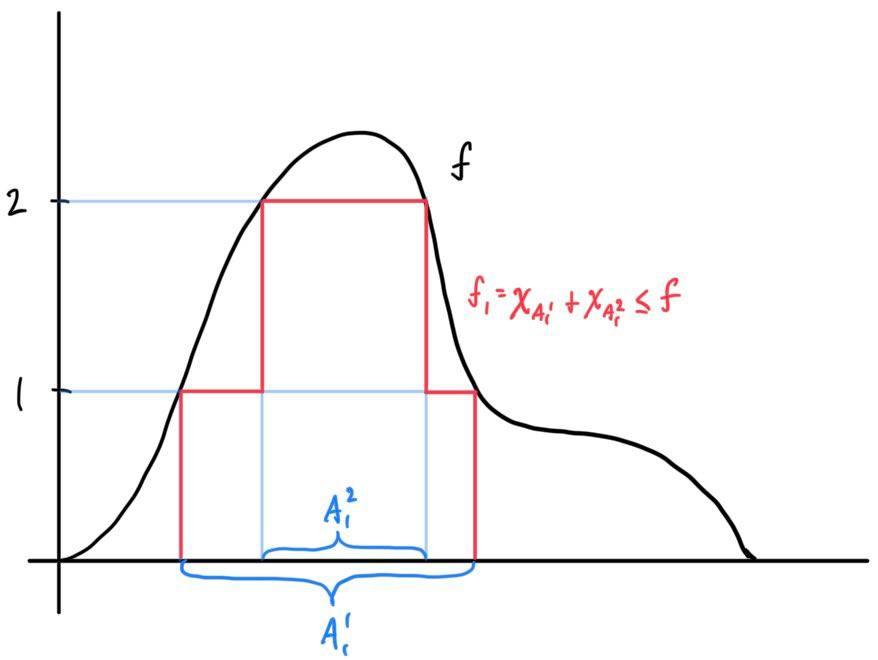
\includegraphics[scale=0.23]{img/Lebesgue_1.jpg}
    \end{center}
    Doing this again with finer subintervals of the codomain gives us, with $f_2 = \chi_{A_2^1} + \chi_{A_2^2} + \chi_{A_2^3} + \chi_{A_2^4} \leq f$. 
    \begin{center}
      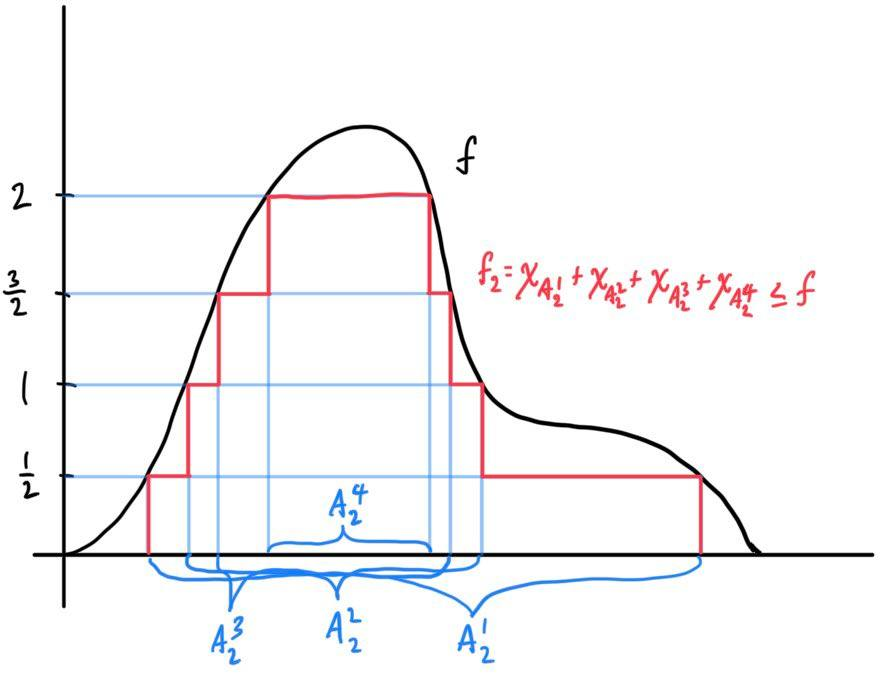
\includegraphics[scale=0.23]{img/Lebesgue_2.jpg}
    \end{center}
    and in general, we have $f_k = \sum_{j=1}^\infty \frac{1}{2^{k-1}} \chi_{A^j_k}$. But we said a simple function is a \textit{finite} sum, and if $\infty$ is in the range of $f$, then this becomes a problem. We can quickly fix this by just truncating the summation at a certain point in the codomain ($f_1$ only considers intervals up to $1$, $f_2$ up to $2$ and so on), ultimately giving us 
    \begin{equation}
      f_k = \sum_{j=1}^{k 2^{k-1}} \frac{1}{2^{k-1}} \chi_{A^j_k} 
    \end{equation}
  \end{proof}



\end{document}

